% Please make sure you insert your
% data according to the instructions in PoSauthmanual.pdf
\documentclass[a4paper,11pt]{article}
\usepackage{pos}
\usepackage{xcolor}
\usepackage{subcaption} % Modern package for subfigures
\usepackage{graphicx}   % Required for inserting images

\usepackage{bbm}
\newcommand{\dd}{\mathrm{d}}
\newcommand{\wtil}[1]{\widetilde{#1}}
\newcommand{\deint}[2]{\dd^{#1}\;\!\!#2\;}
\newcommand{\br}[1]{\left\langle #1 \right |}
\newcommand{\kt}[1]{\left| #1 \right \rangle}
%
\newcommand\brktt[3]{\left< #1 \right| #2 \left| #3 \right>}
\newcommand{\bkt}[2]{\left \langle #1 |#2 \right \rangle}
\newcommand{\brkt}[2]{\left \langle #1 |#2 \right \rangle}
\newcommand{\eps}{\epsilon}
\newcommand{\cEFT}{$\chi$EFT}
\newcommand{\etal}{\textit{et al.}}
\newcommand{\Li}{\mathrm{Li}}
\newcommand{\LiS}{{}^{6} \mathrm{Li} }
\newcommand{\HeF}{{}^{4} \mathrm{He}}
\newcommand{\HeT}{{}^{3} \mathrm{He}}
\newcommand{\HThree}{{}^{3} \mathrm{H}}
\newcommand{\HT}{{}^{2} \mathrm{H}}
\newcommand\bv[1]{\vec{#1}}
\newcommand{\ques}[1]{\color{red}\textit{ #1 }\color{black}}
\newcommand\ddfrac[2]{\frac{\displaystyle #1}{\displaystyle #2}}
\newcommand{\MeV}{\mathrm{MeV}}
\newcommand{\mev}{\mathrm{MeV}}
\newcommand{\fm}{\mathrm{fm}}
\newcommand{\fmin}{\mathrm{fm}^{-1}}

\title{Scattering Observables from Few-Body Densities and Application
in Light Nuclei}
%% \ShortTitle{Short Title for header}

\author*[a]{Alexander Long}
\author[a]{Harald W. Grie{\ss}hammer}
\author[b]{Andreas Nogga}
\author[b]{Xiang-Xiang Sun}

\affiliation[a]{The George Washington University\\ Washington DC USA}
\affiliation[b]{Name of Andreas' institution here}
% \affiliation[a]{Institution,\\
%   Street number, City, Country}

% \affiliation[b]{Department, University,\\
% Street number, City, Country}

\emailAdd{alexlong@gwu.edu}
\emailAdd{hgrie@gwu.edu}
\emailAdd{a.nogga@fz-juelich.de}
\emailAdd{x.sun@fz-juelich.de}
\abstract{
  The dynamics of scattering on light nuclei is well understood, but its
  calculation is numerically difficult using standard methods.
  Fortunately, using recent developments, the relevant quantities can
  be factored into a product of the $n$-body transition density amplitude (TDA) and
  the interaction kernel of a chosen probe.
  These TDAs depend only on the target, and not the
  probe; they are calculated once and stored.
  The kernels depend on only the probe and not the target, moreover they can be reused for different targets.
  The calculation of the transition densities becomes numerically
  difficult for $n\ge4$, but we discuss a solution through use of a
  renormalization
  group transformation.
  This technique allows for extending the density transition method to $\HeF$
  and $\LiS$.
  Throughout this work, Compton scattering is used as test bed, since its kernel is well-developed,
  but extension to pion-photoproduction and other reactions are discussed as well.
}

\FullConference{The 11th International Workshop on Chiral Dynamics (CD2024)\\
  26-30 August 2024\\
Ruhr University Bochum, Germany\\}

%% \tableofcontents

\begin{document}
\maketitle

\section{Introduction}
\ques{This can be 10 pages. Anything is red is a question or
  something that needs to be fixed.\\~\\ I am a little unclear on how
  much discussion of effective field theories, and general intro
  information is needed here.
}

The transition density method was pioneered by Grie{\ss}hammer \etal\,
\cite{hammer2020}.
We seek to analyze an incoming probe, interacting with an $A$ body target.
This probe therefore, may interact with
$1,2,...,A$ nucleons.
The $n$ nucleons it interacts with we call \textit{active} and $A-n$
it does not we call \textit{spectators}.
The mathematical description of these two parts are completely
separate; the $n$ active nucleons contribute to the $n$-body kernel, and spectator
nucleons contribute to the density.
The $n$-body kernel represents the interaction in the idealized case where the probe interacts
with only the $n$-body system. For example, the one-body kernel of Compton scattering contains exactly the 
same contributions as Compton scattering off a Nucleon.
The complete separation of these two parts means if one has access to
$a$ different kernels and $b$ different TDAs, then
$ab$ different results can be produced.
Figure \ref{fig:onetwobod} provides an example for the case $A=3$.

\begin{figure}[h!]
  \begin{center}
    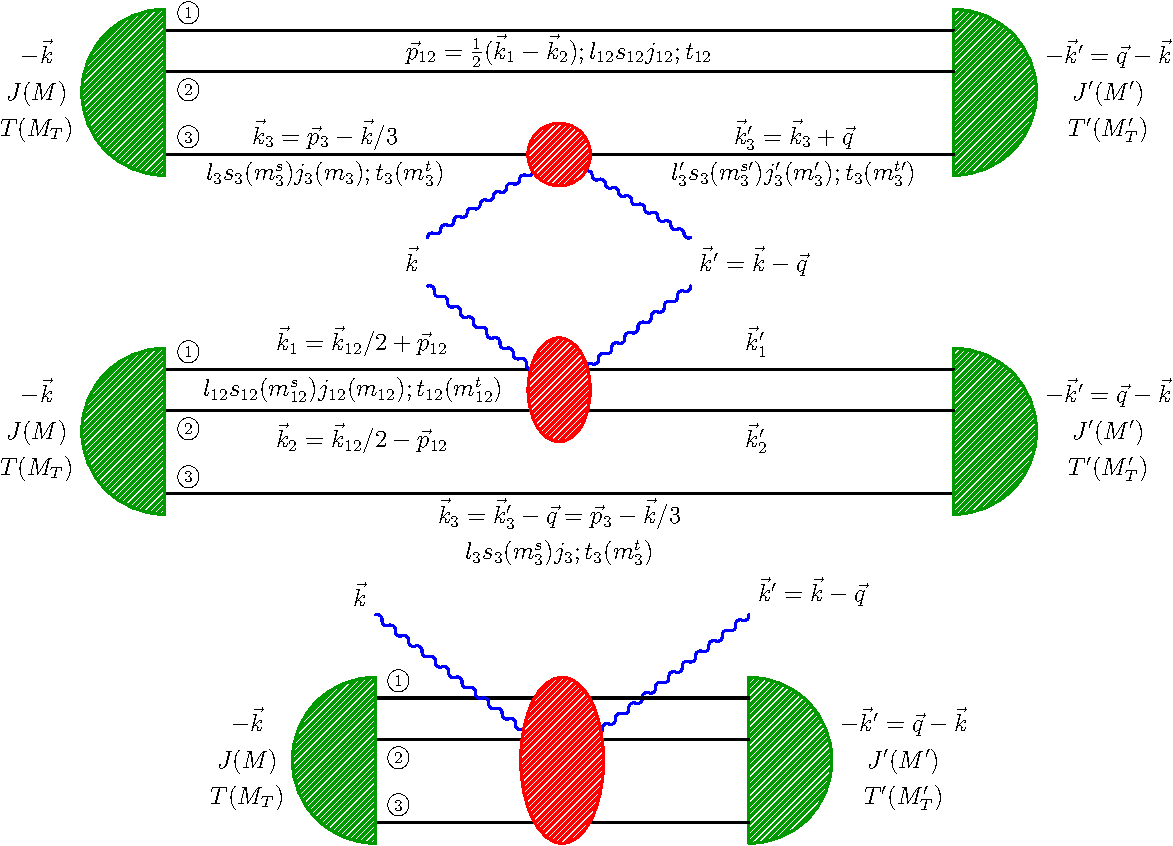
\includegraphics[scale=0.7]{kinematics3He.pdf}
    \caption{Kinematics in the center of mass frame and quantum
      numbers for an $A=3$ system in the case of Compton scattering.
      Generalization to other reactions only changes the kind of
      ingoing/outgoing probe. Top: one-body processes $\hat{O}_3$, center: two-body
      processes $\hat{O}_{2}$, bottom: three-body processes $\hat{O}_{3}$. Green represents the
      densities, and red represents the kernels. From Grie{\ss}hammer \etal
    \cite{hammer2020}}
    \label{fig:onetwobod}
  \end{center}
\end{figure}

For scattering off an $A$ body nucleus, the total scattering
amplitude is given by
\begin{align}
  A_{M}^{M^{\prime} }(\bv{k}, \bv{q})&=\binom{A}{1}\left\langle
  M^{\prime}\right|\hat{O}_{1}^{}(\bv{k}, \bv{q})\left|M\right
  \rangle + \binom{A}{2} \left\langle
  M^{\prime}\right|\hat{O}_{2}^{}(\bv{k}, \bv{q}) \left|
  M\right\rangle\nonumber\\
  &+ \binom{A}{3}\left\langle
  M^{\prime}\right|\hat{O}_{3}^{}(\bv{k}, \bv{q})\left|M\right
  \rangle + \binom{A}{4} \left\langle
  M^{\prime}\right|\hat{O}_{4}^{}(\bv{k}, \bv{q}) \left| M\right\rangle\\
  &+... + \binom{A}{A}\left\langle
  M^{\prime}\right|\hat{O}_{A}^{}(\bv{k}, \bv{q})\left|M\right
  \rangle,\nonumber
\end{align}
where $\hat{O}_i$ is the $i$-body kernel, $M,M'$ is the spin of the target nucleus, and there are
$\binom{A}{i}$ ways for a probe to hit $i$ nucleons. Fortunately,
$\chi$EFT provides a hierarchy of scales which predicts decreasing
contributions for higher order terms for probe energies greater than $\sim 40 \MeV$
\ques{your note says you want a reference here, what do you mean?}
Therefore, the 3-body contribution and higher is negligible at this order, and we simply use
\begin{equation}
  A_{M}^{M^{\prime} }(\bv{k}, \bv{q})=\binom{A}{1}\left\langle
  M^{\prime}\right|\hat{O}_{3}^{}(\bv{k}, \bv{q})\left|M\right
  \rangle + \binom{A}{2} \left\langle
  M^{\prime}\right|\hat{O}_{12}^{}(\bv{k}, \bv{q}) \left|
  M\right\rangle\nonumber\\
\end{equation}
In practice this is enough for accuracy on roughly the 5\% level.
\section{Kernels and Densities}
\ques{I do not think this is specific to the $A=3$ system, but it is taken DIRECTLY from my thesis proposal.}
The one-body and two-body kernel need to be considered separately.
Their form is completely different, and they require a one- and two-body density respectively.
We now write the wave function in the three body system as the
partial-wave decomposition of Jacobi momenta $p_i$ and the relevant
quantum numbers $\alpha$. The wave function in momentum space is given by
\begin{equation}
  \psi_\alpha (p_{12},\, p_3 ) = \bkt{p_{12} p_3 \alpha}{M}.
\end{equation}
The nucleus being described has total angular momentum $J$ and
spin-projection $M$. The momenta are $\bv{p}_{12}= \frac{1}{2}
\left(\bv{k}_1 - \bv{k}_2\right)$ where $ \bv{p}_3 = \bv{k}+
\frac{1}{3} \bv{k}_3 $, and $p_{12} = |\bv{p}_{12}|$ and  $p_{1} =
|\bv{p}_{1}|.$ Here $\bv{k}_i$ are the individual nucleon momenta,
and $\bv{k}$ is the probe momentum in the CM frame. The quantity
$\alpha$ represents all the quantum numbers of the nucleons inside
the nucleus~\cite{hammer2020}
\begin{equation}
  |\alpha\rangle=\left|\left[\left(l_{12} s_{12}\right)
  j_{12}\left(l_{3} s_{3}\right) j_{3}\right] J M,\left(t_{12}
  t_{3}\right) T M_{T}\right\rangle,
\end{equation}
Here $s$, $l$ and $j$ are the spin, orbital and total angular
momentum respectively. The quantum number $s_3$ simply represent the
spin of nucleon 3, whereas $s_{12}$ represents the total spin of the
1-2 subsystem; the quantities $l_{12}$ and $j_{12}$ combine the 1-2
subsystem similarly. Furthermore, $s_{12}$ and $l_{12}$ combine to
$j_{12}$ and likewise for $l_3$, $s_3$ and $j_3$. Finally $j_{12}$
and $j_3$ combine to the total nucleus spin $J$.
The same combinations are done for $t_{12}$, $t_3$ and $T$, with
isospin projection $M_T$. Here $t_3$ and $t_{12}$ are the isospin of
the nucleon labeled 3 and the 1-2 subsystem respectively, $T$ is the
isospin of the entire nucleus and $M_T$ is the number of protons
minus neutrons over 2.
We now seek to describe the scattering amplitudes.

We restrict ourselves to elastic processes, which simplifies the
following discussion by requiring that the probe does not change the
charge of the nucleons \ques{you have a note saying you want me to add "not of the nucleus", I am confused by this}.
For the one body density, the \textit{one-body kernel} of the probe
interaction with nucleon 3 is $O_3$. Leaving nucleons $1$ and $2$ as
spectators~\cite{hammer2020},
\begin{align}
  &\left\langle\bv{k}_{3}^{\prime}\left|\left\langle s_{3} m_{3}^{s
  \prime}\left|\left\langle t_{3} m_{3}^{t
  \prime}\left|\hat{O}_{3}(\bv{k}, \bv{q})\right| t_{3}
  m_{3}^{t}\right\rangle\right| s_{3} m_{3}^{s}\right\rangle\right|
  \bv{k}_{3}\right\rangle \nonumber\\
  &\qquad\qquad\qquad \equiv \delta_{m_{3}^{t \prime} m_{3}^{t}}
  \delta^{(3)}\left(\bv{k}_{3}^{\prime}-\bv{k}_{3}-\bv{q}\right)
  O_{3}\left(m_{3}^{s \prime} m_{3}^{s} m_{3}^{t} ; \bv{k}_{3} ;
  \bv{k}, \bv{q}\right),\label{dirac}
\end{align}
where $m_t$ and $m_t'$ are the isospin of the active nucleon before
and after the interaction (recall $m_t= \pm \frac{1}{2}$ is the proton/neutron).
Symbolically, the matrix element $\hat{O}_3$ is:
\begin{align}
  \left\langle M^{\prime}\left|\hat{O}_{1}(\bv{k}, \bv{q})\right|
  M\right\rangle&=\sum_{\alpha \alpha^{\prime}} \int \mathrm{d}
  p_{12} p_{12}^{2} \mathrm{~d} p_{3} p_{3}^{2} \mathrm{~d}
  p_{12}^{\prime} p_{12}^{\prime 2} \mathrm{~d} p_{3}^{\prime}
  p_{3}^{\prime 2}
  \psi_{\alpha^{\prime}}^{\dagger}\left(p_{12}^{\prime}
  p_{3}^{\prime}\right) \psi_{\alpha}\left(p_{12} p_{3}\right)\nonumber \\
  &\times\left\langle p_{12}^{\prime}
  p_{3}^{\prime}\left[\left(l_{12}^{\prime} s_{12}^{\prime}\right)
    j_{12}^{\prime}\left(l_{3}^{\prime} s_{3}\right)
  j_{3}^{\prime}\right] J^{\prime} M^{\prime}\left(t_{12}^{\prime}
  t_{3}\right) T^{\prime} M_{T}\right| \hat{O}_{1}(\bv{k}, \bv{q})
  \label{onebodFull}\\
  &\qquad\qquad\left|p_{12} p_{3}\left[\left(l_{12} s_{12}\right)
  j_{12}\left(l_{3} s_{3}\right) j_{3}\right] J M\left(t_{12}
t_{3}\right) T M_{T}\right\rangle.\nonumber
\end{align}
The central result is that up to relativistic corrections, this can
be written as:
\begin{align}
  \left\langle M^{\prime}\left|\hat{O}_{1}(\bv{k}, \bv{q})\right|
  M\right\rangle=\sum_{\substack{m_{3}^{s \prime}\,
  m_{3}^{s}\\m_3^t}}\hat{O}_{1}\left(m_{3}^{s \prime} m_{3}^{s},
  m_{3}^{t} ;  \bv{k}, \bv{q}\right) \rho_{m_{3}^{s \prime}
  m_{3}^{s}}^{m_3^{t} M_{T}, M^{\prime} M}(\bv{k}, \bv{q})\label{onebodyOrig}\;.
\end{align}
Here $\rho$, is the \textit{one-body transition density amplitude}
for the nucleus which was discussed previously and can truly be
interpreted as the probability amplitude that nucleon $m_3^t$ absorbs
momentum $\bv{q}$, changes its spin projection from $m_s^3$ to
$m_s^{3'}$ and changes the spin-projection of the nucleus from $M$ to
$M'$. Its operator form is
\begin{equation}
  \rho_{m_{3}^{\prime} m_{3}^{s}}^{m_{3}^{t} M_{T}, M^{\prime}
  M}(\bv{k}, \bv{q})=\left\langle M^{\prime}\right.\left|s_{3}
  m_{3}^{s \prime}, t_{3} m_{3}^{t}\right\rangle
  \mathrm{e}^{\mathrm{i} \frac{2}{3} \bv{q} \cdot
  \bv{r}_{3}}\left\langle s_{3} m_{3}^{s}, t_{3}
  m_{3}^{t}\right|\left. M\right\rangle\label{onebodydens}.
\end{equation}
The two body case works similarly, and results in
\begin{equation}
  \left\langle M^{\prime}\left|\hat{O}_{2}\right| M\right\rangle =
  \sum_{\alpha_{11}^{\prime}, \alpha_{12}} \int \mathrm{d} p_{12}\:
  p_{12}^{2} \mathrm{~d} p_{12}^{\prime}\: p_{12}^{\prime 2}\;
  O_{2}^{\alpha_{12}^{\prime} \alpha_{12}}\left(p_{12}^{\prime},
  p_{12}\right) \rho_{\alpha_{12}^{\prime} \alpha_{12}}^{M_{T},
  M^{\prime} M}\left(p_{12}^{\prime}, p_{12} ; \bv{q}\right)\label{twobody}\;.
\end{equation}
This is the two-body equivalent to \eqref{onebodyOrig}.
There is an expression analogous to \eqref{onebodFull} but, it is non-trivial and for our purposes non-enlightening.
This two-body density $\rho_{\alpha_{12}^{\prime}
\alpha_{12}}^{M_{T}, M^{\prime} M}$ is of course completely distinct
from the one-body density. 
However, just like the one-body case it can also be interpreted as a probability density.
It is dependent on the incoming and outgoing quantum numbers
$\alpha_{12}$ and $\alpha_{12}'$ of the 1-2 system, and also on the
relative momenta of the two nucleons which are integrated over.
As a result, the total file size for the two nucleon densities are on
the order of a few GB per energy and angle, whereas those of the one
nucleon densities are on the order of a few KB.
Importantly, $\rho$ can be computed generically from a nuclear
potential, such as the chiral SMS potential
without reference to the kernel $\hat{O}_3$ or $\hat{O}_{12}$
\cite{Reinert2018}.
\ques{Maybe this is too much detail. Later if we run out of space we can cut the intro discussion and just use the definitions
of the one/two body operators.}

\section{SRG Transform}
Previous work using the TDA formalism has analyzed
$\HeT$ and $\HeF$, but to extend this $\LiS$ involves many body
interactions which are much more complicated, and numerically expensive
\cite{hammer2020, hammer4He}.
To make the calculation of a TDA feasible for $A=6$, a \textit{similarity renormalization group} (SRG) transformation
is used \cite{SRG}.
When using nuclear potentials, we approximate the potential to be zero 
outside a certain cutoff $\Lambda$, and therefore neglect it in our calculation.
In general, a nuclear potential, such as the chiral SMS potential does
not fall off quickly for high momenta, meaning we would have to
extend the cutoff much further than we would like, which in turn
increases computational cost.
The SRG transform is a unitary transformation that allows us to
move all the dependence into the low momentum region, thereby decreasing the
lowest possible value of the cutoff, which in turn makes
calculation for $A=6$ converge significantly faster.
The SRG transformation can be thought of as a local averaging or
smoothing out of the potential, resulting in decreased ``resolution''
has the SRG is applied.
\begin{figure}[h]
  \centering
  \begin{subfigure}{0.45\textwidth}
    \centering
    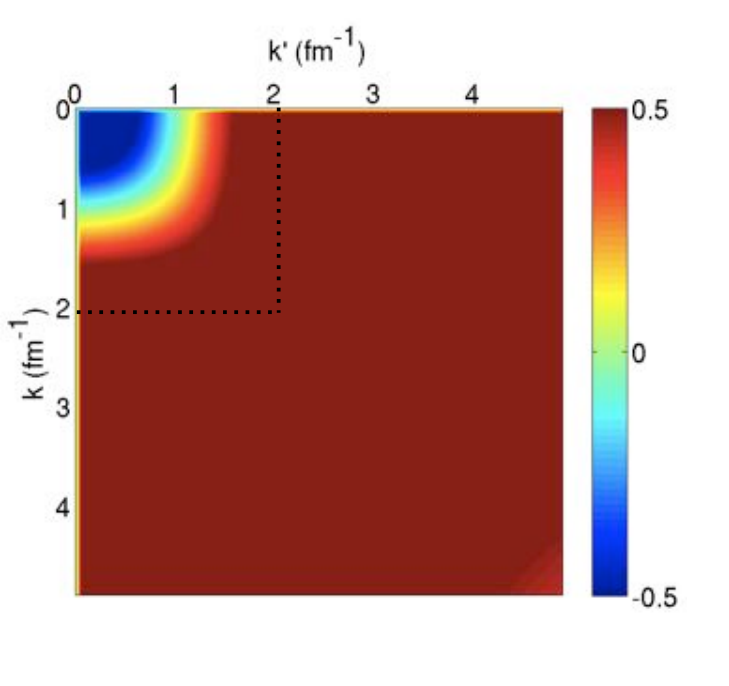
\includegraphics[width=\linewidth]{HighRes.png}
    \caption{High Resolution (before much SRG is applied) }
    \label{fig:highres}
  \end{subfigure}
  \hfill
  \begin{subfigure}{0.45\textwidth}
    \centering
    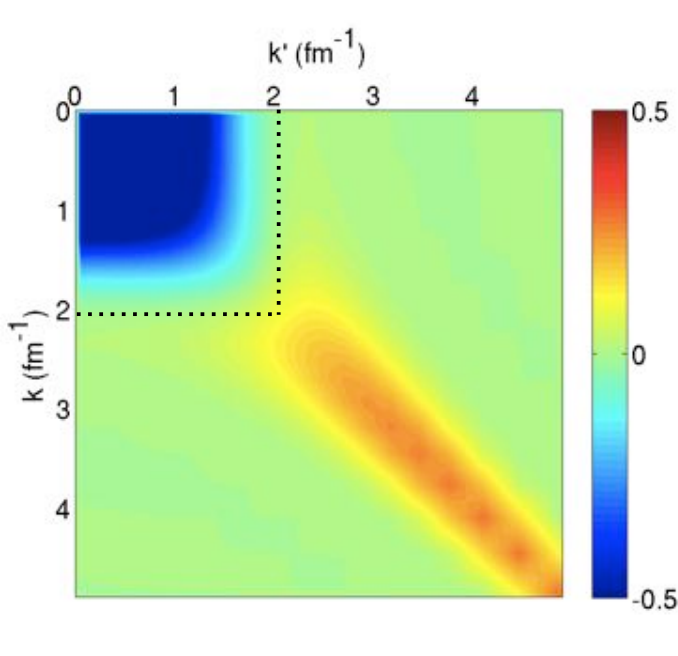
\includegraphics[width=\linewidth]{LowRes.png}
    \caption{Low Resolution (evolved)}
    \label{fig:lowres}
  \end{subfigure}
  \caption{Nuclear potentials $V(k,k')$. Figures from Kai Hebeler:
    ``Chiral Effective Field Theory and Nuclear Forces:
  overview and applications'' presentation at TALENT school at MITP 2022}
  \label{fig:SRGtransform}
\end{figure}
In the under-evolved, high resolution figure \ref{fig:highres} one can
see the potential does not go to zero quickly whereas once the
transformation is applied in figure \ref{fig:lowres} it does. As a
result a cutoff can be made at \ques{I like calling it $k$ here, not $\Lambda$} $k,k'=2 \mathrm{fm}^{-1}$ without
losing much accuracy. In the example above, the under-evolved
potential had to be considered up to $k,k'=5\mathrm{fm}^{-1}$, this means an efficiency
gain proportional to the areas of each, for a factor of $(5/2)^2=6.25$.

However, this creates another problem: the SRG transform creates a
change in the physical meaning of the free variables.
To understand this, let us first consider an example the reader is
certainly more familiar with - a Fourier transformation which changes
a potential from position to momentum space.
\begin{equation}
  V(\vec{r},\vec{r}\,')= \br{r'} V \kt{r}=
  \int \dd^3p\, \dd^3p' \brkt{r'}{p'} \br{p'}V\kt{p} \brkt{p}{r}\\
  =V(\vec{p},\vec{p}\,')
\end{equation}
After the transform, our free variables have different physical
meaning. In fact, any unitary transform also transforms the coordinates.
\begin{align}
  \br{p'}V\kt{p} &= \br{p'} \mathbbm{1} V \mathbbm{1} \kt{p}\nonumber\\
  &= \br{p'} U^\dag U V U^\dag U \kt{p}\nonumber\\
  &= \left(\br{p'} U^\dag\right)\;\left( U V U^\dag\right)\;\left( U
  \kt{p}\right)\\
  &= \br{\widetilde{p}\,'} V_{eff}
  \kt{\widetilde{p}}=V_{eff}(\widetilde{p},\widetilde{p}\,')\nonumber
\end{align}
So calling the free variables in an SRG-transformed potential
``momenta'' to some degree is abuse of notation.
They are not physical states \ques{you have a note here "variables are states?" what do you mean by this?} in the sense that $\wtil{p}=50 \MeV$
does not correspond to a state of $50 \,\MeV$ an experimentalist can prepare.
The Lagrangians that generate the Feynman diagrams in the kernel, however,
depend on physical momenta, and therefore we cannot directly use an SRG 
evolved potential in the non-SRG evolved kernel.
To solve this, previous work with SRG transformations has transformed
Lagrangians and therefore the kernels into the SRG evolved space as well. However, in
the case of the density formalism this would mean adding SRG
information into the kernel, thereby breaking kernel-density independence.
Additionally, the SRG transformation can take many different forms; 
the state-of-the-art transformation has
changed over the years, and we wish to allow for these developments
without having to re-write the kernel code \ques{add reference}.
Therefore we have chosen to apply an inverse
transformation to the densities\ques{maybe cite Xiang-Xiang, depending on what they want}.

This work was begun with the highest nucleon number system we can
calculate densities for without an SRG transformation, which is
$\HeF$. In this way we gained confidence in $\HeF$ before moving
to the more complex $\LiS$.
\ques{Are they not publishing a paper on this? How do I credit
Xiang-Xiang effectively?}
\begin{figure}[h!]
  \begin{center}
    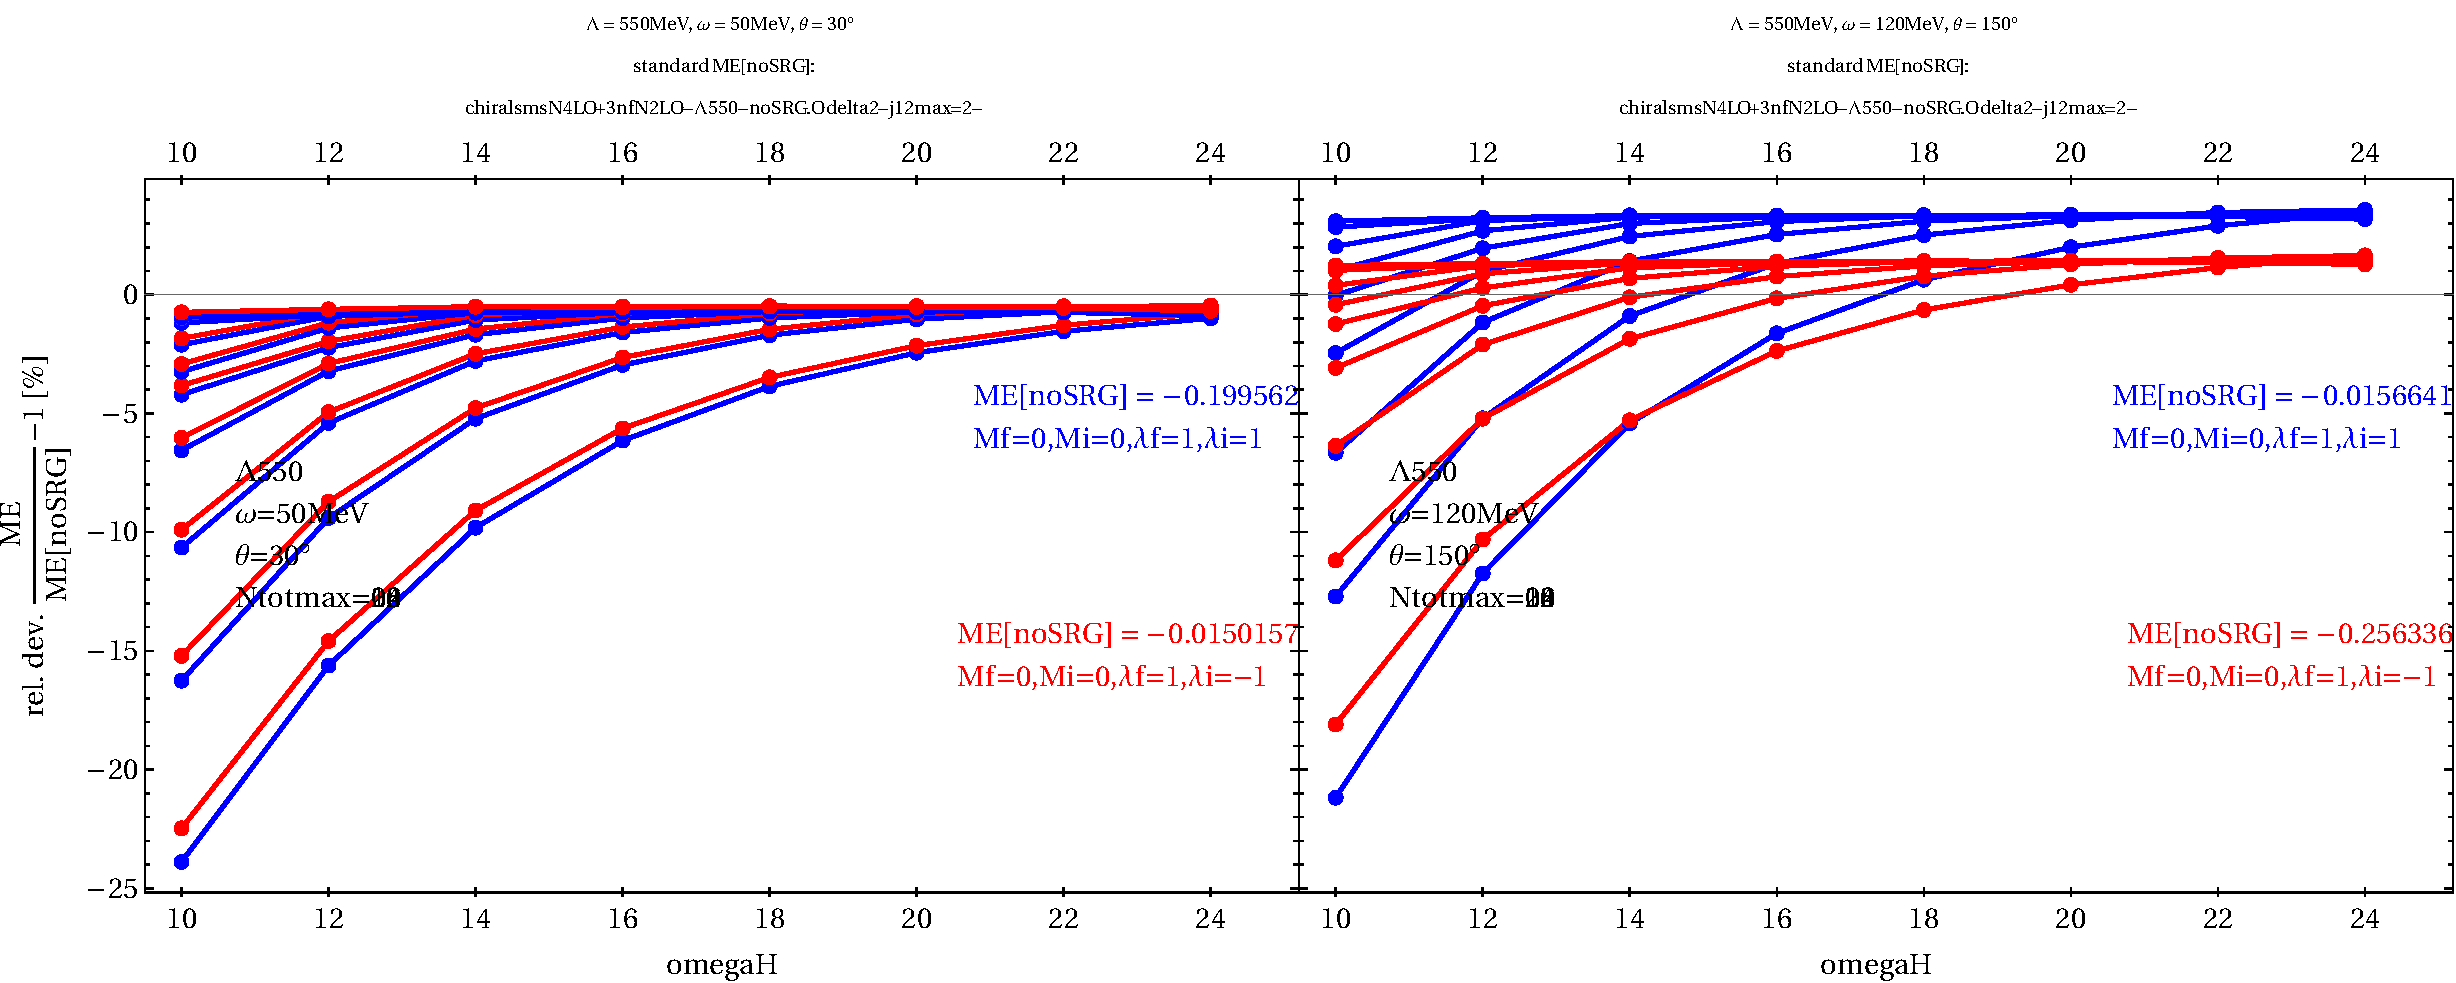
\includegraphics[width=\linewidth]{SRG-Converge-Double.pdf}
    \caption{A convergence plot for $\HeF$\, Compton scattering
    showing the relative deviation of the matrix elements (ME) of the reaction.\ques{What about an Ntotmax convergence plot? also I fear I don't understand something or this plot is mislabeled, why does strictly increasing omegaH decrease error}}
    \label{fig:SRGConverge4He}
  \end{center}
\end{figure}
In figure \ref{fig:SRGConverge4He}, we see the effectiveness of the results in the $\HeF$ case.
The SRG transformation uses the harmonic oscillator basis,
with `omegaH` on the $x$-axis representing the width of the harmonic
oscillator potential, and `Ntotmax` the quantum numbers of the highest harmonic oscillator excitation used.
The harmonic oscillators form a complete basis state for this system.
\ques{I'm writing this next part as if the plot above actually has Ntotmax on the x-axis.}
Expansion to $N=\infty$, $\Lambda_{\text{cutoff}}=\infty$ would result in perfect agreement.
The truncation to finite $\Lambda$ results in induced many-body forces, but this effect is small.
The truncation to finite $N$ is much more significant, and drastically effects the computational resources required.
The figure \ref{fig:SRGConverge4He} shows the combined effect of both of these truncations; we expect the deviation to decrease as $N$ increases, and importantly for our analysis, this shows what value of $N$ is required.
With this completed we have now moved to $\LiS$.
This is of much interest experimentally since this target is stable solid at room temperature,
it is therefore easy to conduct an experiment on, even to high precision due to its relatively large
cross section.
\ques{$\LiS$ results go here.}
\section{Analyzing Different Interactions}
We are of course interested in Compton scattering but we also with to extend the density
formalism to other processes. In particular pion-photoproduction, and
pion-pion scattering are of interest.
Fortunately their kernels share remarkable similarity since there are
only so many ways for one particle to go in and one to go out.
\subsection{Compton Scattering}
Compton scattering allows for extraction of the nucleon polarizabilites.
$\alpha_{E1}, \beta_{M1}$, a subject of much experimental interest. 
These parameters quantify the stiffness of a nucleus, and enter in the Hamiltonian via
\begin{equation}
    \mathcal{H}=-4\pi \left( \frac{1}{2} \alpha_{E1} \bv{E}^2 + \frac{1}{2} \beta_{M1} \bv{H}^2\right)
\end{equation}
There are many experiments on $\LiS$, yet as of now there is no theory prediction \cite{60MeV,86MeV}. We seek to fill this gap.


\subsection{Pion-Photoproduction}
For the pion-photoproduction one-body kernel, we use the results of scattering on a single nucleon, $\gamma N \to \pi N$ which has
been studied extensively \cite{pionphoto, Rijneveen2021,Workman2012,Briscoe2023}.
Its differential cross section can be decomposed in terms of the
electric and magnetic multipoles $E_{l\pm}, M_{l\pm}$ which are angle
independent  \cite{pionphoto}.
There have been many experimental results over the years
which measure these multipoles to high order and with good precision
such as ``Unified Chew-Mandelstam SAID analysis...'' Workman \etal \cite{multipolePionPion}.
The scattering matrices $\mathcal{M}$ which result from this are exactly what enters as $\hat{O}_3$ in equation (\ref{onebodyOrig}). 
This solves a significant problem since calculation of the one-body pion-photoproduction kernel to high accuracy directly through Feynman diagrams requires including many terms in the chiral expansion due to the proximity of the $\Delta(1232)$ resonance at $\sim 200\MeV$ \cite{chiralpionphoto}.

The two-body contributions do not easily decompose into multipole interactions, therefore we preform the calculation through expansions in the chiral Lagrangian through calculation of Feynman diagrams.
At threshold energy this reaction kernel has been analyzed by Lenkewitz \etal \cite{L2011, L2013}.
We now have a numerically stable result for $\HeT$ and seek to extend this to new targets.
\ques{Include some numbers}
\subsection{Pion-Pion scattering and other reactions}
The pion-pion scattering kernel is similar to the pion-photoproduction kernel.
Beane \etal has developed the pion-pion kernel at threshold for both one-body and two-body interactions \cite{Beane2003}.
We may extend this to finite energy\ques{You have a note here I cannot make out, it looks like "cheis as well?".} 
Once the pion-photoproduction and pion-pion scattering kernels have successfully been developed, we will instantly be able to calculate all of these reactions on targets previously analyzed in the density formalism since we already have produced the densities required.
In particular, we will calculate all of these reactions with the targets $\HThree$, $\HeT$, $\HeF$, and $\LiS$.\ques{are we actually doing $\HThree$?} 
\section{Conclusion}


\begin{thebibliography}{99}
  \bibitem{hammer2020}
  H. W. Grie{\ss}hammer, J. A. McGovern, A. Nogga, and D. R.
  Phillips, ``Scattering Observables from One- and Two-body
  Densities: Formalism and Application to $\gamma^3$ Scattering,''
  \textit{Few-Body Systems}, vol. 61, no. 4, Nov. 2020. DOI:
  \href{https://doi.org/10.1007/s00601-020-01578-w}{10.1007/s00601-020-01578-w}.

  \bibitem{Reinert2018}
  P. Reinert, H. Krebs, and E. Epelbaum, ``Semilocal momentum-space
  regularized chiral two-nucleon potentials up to fifth order,''
  \textit{The European Physical Journal A}, vol. 54, no. 5, May 2018.
  DOI:
  \href{http://dx.doi.org/10.1140/epja/i2018-12516-4}{10.1140/epja/i2018-12516-4}.
  \bibitem{hammer4He}
  H. W. Griesshammer, J. Liao, J. A. McGovern, A. Nogga, and D. R.
  Phillips, ``Compton Scattering on 4He with Nuclear One- and
  Two-Body Densities,''
  \href{https://arxiv.org/abs/2401.16995}{arXiv:2401.16995}.

  \bibitem{SRG}
  S. Szpigel and R. J. Perry, ``The Similarity Renormalization
  Group,''.
  \href{https://arxiv.org/abs/hep-ph/0009071}{arXiv:hep-ph/0009071}.

  \bibitem{pionphoto}
  R. L. Walker, ``Phenomenological Analysis of Single-Pion
  Photoproduction,'' \textit{Phys. Rev.}, vol. 182, no. 5, pp.
  1729--1748, Jun. 1969. DOI:
  \href{https://link.aps.org/doi/10.1103/PhysRev.182.1729}{10.1103/PhysRev.182.1729}.

  \bibitem{multipolePionPion}
  R. L. Workman, M. W. Paris, W. J. Briscoe, and I. I. Strakovsky,
  ``Unified Chew-Mandelstam SAID analysis of pion photoproduction
  data,'' \textit{Phys. Rev. C}, vol. 86, no. 1, p. 015202, Jul.
  2012. DOI:
  \href{https://link.aps.org/doi/10.1103/PhysRevC.86.015202}{10.1103/PhysRevC.86.015202}.

\bibitem{chiralpionphoto}
N. Rijneveen, A. M. Gasparyan, H. Krebs, and E. Epelbaum, ``Pion photoproduction in chiral perturbation theory with explicit treatment of the $\Delta(1232)$ resonance,''  \href{https://arxiv.org/abs/2108.01619}{arXiv:2108.01619}.

\bibitem{L2011}
M. Lenkewitz, E. Epelbaum, H.-W. Hammer, and U.-G. Meißner, ``Neutral pion photoproduction off $^3$H and $^3$He in chiral perturbation theory,'' \textit{Physics Letters B}, vol. 700, no. 5, pp. 365–368, Jun. 2011. DOI: \href{http://dx.doi.org/10.1016/j.physletb.2011.05.036}{10.1016/j.physletb.2011.05.036}.

\bibitem{L2013}
M. Lenkewitz, E. Epelbaum, H.-W. Hammer, and U.-G. Meissner, ``Threshold neutral pion photoproduction off the tri-nucleon to $O(q^4)$,'' \textit{The European Physical Journal A}, vol. 49, no. 2, Feb. 2013. DOI: \href{http://dx.doi.org/10.1140/epja/i2013-13020-1}{10.1140/epja/i2013-13020-1}.

\bibitem{86MeV}
L. S. Myers, M. W. Ahmed, G. Feldman, A. Kafkarkou, D. P. Kendellen, I. Mazumdar, J. M. Mueller, M. H. Sikora, H. R. Weller, and W. R. Zimmerman, ``Compton scattering from $^{6}\mathrm{Li}$ at 86 MeV,'' \textit{Phys. Rev. C}, vol. 90, no. 2, p. 027603, Aug. 2014. DOI: \href{https://link.aps.org/doi/10.1103/PhysRevC.90.027603}{10.1103/PhysRevC.90.027603}.

\bibitem{60MeV}
L. S. Myers, M. W. Ahmed, G. Feldman, S. S. Henshaw, M. A. Kovash, J. M. Mueller, and H. R. Weller, ``Compton scattering from $^{6}$Li at 60 MeV,'' \textit{Phys. Rev. C}, vol. 86, no. 4, p. 044614, Oct. 2012. DOI: \href{https://link.aps.org/doi/10.1103/PhysRevC.86.044614}{10.1103/PhysRevC.86.044614}.

\bibitem{Beane2003}
S. R. Beane, V. Bernard, E. Epelbaum, U.-G. Meißner, and D. R. Phillips, ``The S-wave pion–nucleon scattering lengths from pionic atoms using effective field theory,'' \textit{Nuclear Physics A}, vol. 720, no. 3–4, pp. 399–415, Jun. 2003. DOI: \href{http://dx.doi.org/10.1016/S0375-9474(03)01008-X}{10.1016/S0375-9474(03)01008-X}.

\bibitem{Rijneveen2021}
N. Rijneveen, A. M. Gasparyan, H. Krebs, and E. Epelbaum, ``Pion photoproduction in chiral perturbation theory with explicit treatment of the $\Delta(1232)$ resonance,'' 2021. Available: \href{https://arxiv.org/abs/2108.01619}{arXiv:2108.01619}.

\bibitem{Workman2012}
R. L. Workman, M. W. Paris, W. J. Briscoe, and I. I. Strakovsky, ``Unified Chew-Mandelstam SAID analysis of pion photoproduction data,'' \textit{Phys. Rev. C}, vol. 86, no. 1, p. 015202, Jul. 2012. DOI: \href{https://link.aps.org/doi/10.1103/PhysRevC.86.015202}{10.1103/PhysRevC.86.015202}.
\bibitem{Briscoe2023}
W. J. Briscoe, A. Schmidt, I. Strakovsky, R. L. Workman, and A. \ifmmode \check{S}\else \v{S}\fi{}varc, ``Extended SAID partial-wave analysis of pion photoproduction,'' \textit{Phys. Rev. C}, vol. 108, no. 6, p. 065205, Dec. 2023. DOI: \href{https://link.aps.org/doi/10.1103/PhysRevC.108.065205}{10.1103/PhysRevC.108.065205}.

\end{thebibliography}

\end{document}
